\documentclass[a4paper, 15pt]{article}
\usepackage[left=0.85in, right=0.85in, top=0.5in, bottom=0.95in]{geometry}
\usepackage[T1]{fontenc}
\usepackage[utf8]{inputenc}
\usepackage[italian]{babel}
\usepackage[none]{hyphenat} % no sillabazione 
\usepackage{multicol} %testo su più colonne
\usepackage{enumerate}
\usepackage{enumitem}
\usepackage{mdwlist} %suspend enumerate \suspend{} \resume{}
\usepackage{lipsum} %testo random per verifica \lipsum
\usepackage{graphicx, nicefrac}
\usepackage{wrapfig2}
\usepackage{amsmath}
\usepackage{mathtools}
\usepackage{amssymb}
\usepackage{amsthm} %teoremi e dimostrazioni e definizioni
\usepackage{cases}
\usepackage{gensymb} %simboli come ° = \degree  etc etc
\usepackage{cancel} %permette di fare semplificazioni utilizzando il comando \cancel{expression}
\usepackage{subcaption}
\usepackage{hyperref}
\hypersetup{
	colorlinks=true,
	linkcolor=blue,    
	urlcolor=blue,
	%pdfpagemode=FullScreen, %il pdf generato non si avvia a schermo intero
}
\urlstyle{same}
\usepackage{changepage}
\usepackage{lastpage, epstopdf}
\usepackage{fancyhdr}
\usepackage{tcolorbox}
%\usepackage{background} %non utilizza lo sfondo con "draft"
\usepackage{color} % testo colorato \textcolor{'ColorCode'}{'testo'}
\usepackage{setspace} % in questo modo posso settare lo spoazio dell'indice \begin{spacing}{0.95}

\usepackage{changepage}
\usepackage{lastpage, epstopdf}
\usepackage{fancyhdr}
\usepackage{tcolorbox}
%\usepackage{background}
\usepackage{tikz} %disegni e mappe
\usetikzlibrary{patterns}
\usepackage{pgfplots}
\pgfplotsset{compat=1.15}
\usepackage{mathrsfs}
\usetikzlibrary{arrows,decorations.markings}
\raggedbottom
\setlength{\parindent}{0pt}
%%%%%%%%%%%%%%%%%%%%%%%%%%%%%%%%%%%%%%%%%%%% SIUNITX 
\usepackage{siunitx}
	
%========TEOREMI========%
\newtheorem*{thm}{Teorema}
\newtheorem*{en}{Enunciato}
\newtheorem*{definizione}{Definizione}
\newtheorem*{cor}{Corollario}
	
	
	
	%========OPERATORI&COMANDI========%
\DeclareMathOperator{\rk}{rk}
\DeclareMathOperator{\im}{Im}
\DeclareUnicodeCharacter{20AC}{\EUR}
\newcommand{\cmark}{\ding{51}}
\newcommand{\xmark}{\ding{55}}
\newcommand{\compresslist}{ % Define a command to reduce spacing within itemize/enumerate environments, this is used right after \begin{itemize} or \begin{enumerate}
				\setlength{\itemsep}{1pt}
				\setlength{\parskip}{0pt}
				\setlength{\parsep}{0pt}
			}
\newcommand{\ra}[1]{\renewcommand{\arraystretch}{#1}} %stretcho le tabelle
			
%\renewcommand{\arraystretch}{2.5} % Da copiaincollare prima di ambienti array per ampliarli un po'
%\setlength{\jot}{10pt} % affecting the line spacing in the environment SPLIT
			
\begin{document}
				\setcounterpageref{secnumdepth}{0}	
				\tableofcontents 
				\newpage
				
\part{3.STATISTICA}
\section{Introduzione}	
\begin{adjustwidth}{2in}{}
	 	La misura di una grandezza fisica riportata mediante un numero esatto è scientificamente priva di senso se non si precisa l’entità dell’errore da cui essa può essere affetta. La norma UNI 4546 definisce infatti la misura come un’informazione costituita da un numero, da un’incertezza e da un'unità di misura.
	 	
	 	Esistono due tipo di errori.
	 	\begin{itemize}
	 		\item \textbf{Casuali}: non controllabili, risultato di una misura meno la media che risulterebbe da un numero infinito di misurazioni del misurando effettuate sotto condizioni di ripetibilità [VIM 3.13].
	 		
	 		Potendo essere di entrambi i segni possono determinare una sottostima od una sovrastima del misurando.
	 		
	 		\item \textbf{Sistematici}: controllabili ed eliminabili se noti, media che risulterebbe da un numero infinito di misurazioni del misurando effettuate sotto condizioni di ripetibilità meno il valore vero del misurando [VIM 3.14].
	 		
	 		Influiscono sulla misurazione sempre nello stesso modo e hanno sempre lo stesso segno qualunque misura del misurando venga effettuata.
	 	\end{itemize}
	 	Agli errori sistematici è associata la \textbf{giustezza}, questa aumenta quanto minore diviene lo scostamento tra valore vero ed il valore medio delle misure fatte.\newline
	 	
	 	 Agli errori casuali è associata la \textbf{precisione}: una misura è più precisa quanto è minore lo scostamento tra la singola misura e la media di tutte le misurazioni fatte. 
	 	 
	 	 L’entità di tale scostamento rappresenta l’incertezza associata alla misura.\newline
	 	 
	 	 \begin{center}
	 	 	\textbf{LA SEGUENTE TRATTAZIONE È PRIVA DI ERRORE SISTEMATICO}\newline
	 	 \end{center} 
	 	 
	 	 Lo scopo così che si prefigge la statistica sarà quello di capire come l'incertezza influenzi il valore vero attraverso l'errore casuale. 
	 	 
	 	 L’analisi dell’incertezza si basa su due concetti fondamentali:
	 	 \begin{enumerate}
	 	 	\item \textbf{Distribuzione di probabilità dell'errore}\newline 
	 	 	Risponde alle domande:
	 	 	\begin{itemize}
	 	 		\item Qual è la probabilità che ho nel commettere l'errore?
	 	 		\item Qual è la probabilità che ho che la misura cada nell'intervallo che voglio?
	 	 	\end{itemize}
 	 	Quantifica perciò la probabilità che si verifichi un errore di entità fissata rispetto al valor vero di una misura.
 	 	
 	 	 Equivalentemente, quantifica l'entità dell'errore sulla misura corrispondente ad una data percentuale di probabilità.
 	 	 
 	 	 \item \textbf{Campione VS Popolazione} \newline 
 	 	 Mentre la \underline{popolazione} è identificata da tutte le possibili misura che si potrebbero effettuare, il \underline{campione} sono null'altro le misure realmente ottenute.
	 	 \end{enumerate}
 	 	L’analisi statistica degli errori utilizza sempre un modello matematico che descrive la distribuzione degli errori commessi nelle misure effettuate. Solo mediante la conoscenza di tale distribuzione è possibile calcolare la probabile differenza tra la media $\overline{X}$ dei valori di una serie di campioni $ x_i $ e quella della popolazione $\mu$. 
\newpage 	 	
 	 	Si definiscono:
 	 	\begin{itemize}
 	 		\item Campione
 	 		\[x = x_i \dots x_n\]
 	 		
 	 		\item Numero di campioni 
 	 			 	\[n\]
 	 			 	
 	 		\item Media aritmetica del campione $X$
 	 			 	\[\overline{x} = \sum_{i=1}^{n}{x_i\over n}\]
 	 			 	
 	 		\item Media della popolazione \newline 
 	 		\[\mu\]
 	 		Non calcolabile: non ho la popolazione ma solo il campione. 
 	 		
 	 		Se la popolazione uguaglia il campione \(\mu = \overline{X}\)
 	 		
 	 		\item Scarto della i-esima misura dalla media
 	 		\[\xi_i = x_i - \overline{x}\]
 	 		Per definizione di media, la somma degli scarti è sempre nulla. 
 	 		\[\sum_{i=1}^{n}\xi_i = \sum_{i=1}^{n}\left(x_i - \overline{x}\right) = \sum_{i=1}^{n}\left(x_i - \sum_{i=1}^{n}{x_i\over n}\right) = 0 \]
 	 		
 	 		\item Errore della i-esima misura
 	 		\[\varepsilon_i = x_i -\mu\]
 	 		
 	 		\item Errore medio
 	 		\[\overline{\varepsilon} = \overline{x} - \mu\]
 	 		
 	 		\item Deviazione standard della popolazione
 	 		\[\sigma_x \sqrt{\dfrac{\sum_{i=1}^{n}\varepsilon^2_i}{n}}\]
 	 		
 	 		\item Deviazione standard del campione
 	 		\[s_x \sqrt{\dfrac{\sum_{i=1}^{n}\xi^2_i}{n-1}}\]
 	 		Questo parametro è fondamentale poiché, nella maggior parte dei casi, per risalire all’incertezza associata ad una misura non sono note né $\sigma$ né $\mu$. \newline
 	 		
 	 		Notare il $-1$ al denominatore, fattore correttivo. Deriva dal fatto che se il campione coincide con la popolazione, è meglio ottenere un'incertezza pari a $0/0$ e quindi indeterminata, che un'incertezza nulla derivante dall'assenza del fattore $-1$, il che è un assurdo fisico dato che l'incertezza è sempre legata alla misura. 
 		\end{itemize}
 \end{adjustwidth}
 \newpage
 \section{Distribuzione dei valori attorno al valor medio: curva di Gauss}
 \begin{adjustwidth}{2in}{}	
 	Sotto le seguenti ipotesi: \(\overline{x} = \mu; s_x = \sigma_x; \) e che tutti gli errori siano casuali ($N\rightarrow\infty$) e quindi considerabili a media nulla, ci si chiede come si distribuisce la misura intorno al valor medio. \newline
	
 	Ci si chiede perciò: se si effettua un’ulteriore misurazione, quale è la probabilità che si trovi un valore pari proprio alla media? Come ci si deve comportare se si trova un valore molto diverso dalla media? Fino a che punto possiamo considerare attendibile anche tale nuovo valore? 
 \begin{figure}[H]
	\centering
	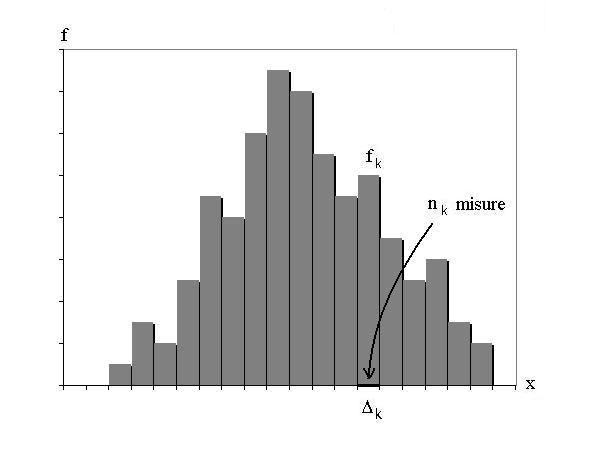
\includegraphics[width=0.5\linewidth]{fig/screenshot001}
	\label{fig:screenshot001}
\end{figure} 	
 	Per rispondere a tali domande si introduce la distribuzione Gaussiana, ovvero, si prendano gli $x_i$ valori ottenuti e li si componga ad istogramma da $x_{min}$ ad $x_{max}$; l'altezza di ogni barra corrisponde alla quantità di misure/valori mentre la base sarà un intervallo di valori $\Delta x$; come questo intervallo diminuisce, l'istogramma presenterà barre sempre più sottili e fine fino ad approssimare una curva.  	
 	\begin{figure}[H]
 		\centering
 		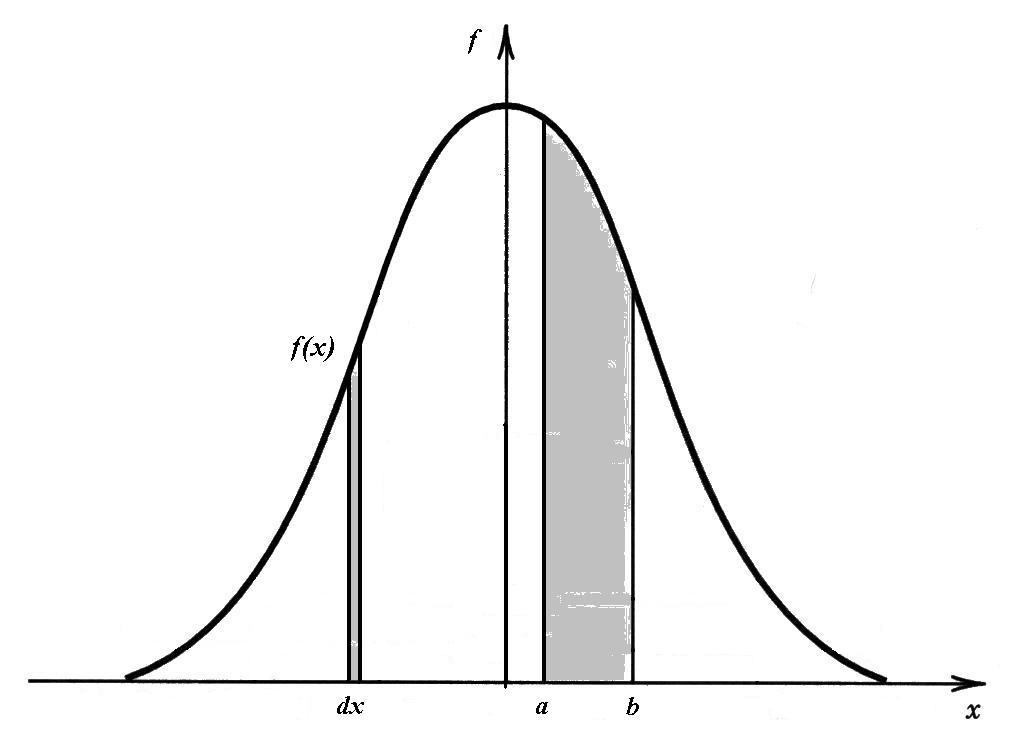
\includegraphics[width=0.5\linewidth]{fig/screenshot002}
 		\label{fig:screenshot002}
 	\end{figure}	
 	Il teorema limite centrale afferma che la distribuzione gaussiana permette di descrivere, in maniera soddisfacente, tutti quei fenomeni fisici caratterizzati dalla sovrapposizione di un elevato numero di effetti deboli indipendenti aventi loro natura statistica a media nulla. Questa distribuzione è anche detta Normale in quanto si suppone, alle volte in modo non corretto, che molti fenomeni tra cui quelli fisici e biologici “normalmente” si distribuiscono secondo la curva gaussiana. 	
 	\[y(x) = \dfrac{1}{\sigma_x\sqrt{2\pi}}e^{\dfrac{(x-\mu)^2}{2\sigma_x^2}}\]
 	Tale funzione, integrata, indicherà la probabilità che una determinata misura caschi all'interno di un determinato intervallo.
 	\[P(x) = \int_{a}^{b}y(x)dx = \int_{a}^{b}\dfrac{1}{\sigma_x\sqrt{2\pi}}e^{\dfrac{(x-\mu)^2}{2\sigma_x^2}}dx\]
	 Come ottengo il $100\%$? Integrando su tutto lo spazio. 
	 \[ \int_{-\infty}^{+\infty}\dfrac{1}{\sigma_x\sqrt{2\pi}}e^{\dfrac{(x-\mu)^2}{2\sigma_x^2}}dx = 1\]
	 La distribuzione normale con media $\mu$ e varianza $ \sigma_x^2 $ si indica con $ N(\mu,\sigma_x $). Al variare di questi due parametri si possono avere infinite curve.\newline 
	 
	 La funzione di densità in esame è simmetrica rispetto alla media ed ha due flessi nei punti $ \mu\pm\sigma_x $.	 	
\begin{figure}[H]
	\centering
	\label{fig:screenshot006}
	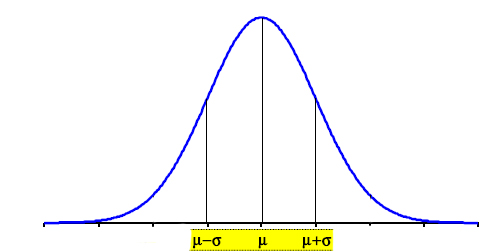
\includegraphics[width=0.5\linewidth]{fig/screenshot006}
\end{figure}
	Si identificano due casistiche per le quali:
	\begin{itemize}
	\item \(\begin{cases}
			\mu_2>\mu_1 \\
			\sigma_{x2}=\sigma_{x1}
		\end{cases}\) la curva è traslata, ha la stessa forma e dimensione ma l'asse di simmetria in un punto diverso. 
\begin{figure}[H]
	\centering
	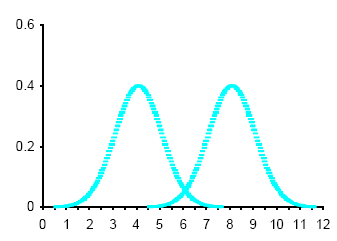
\includegraphics[width=0.3\linewidth]{fig/screenshot004}
	\label{fig:screenshot004}
\end{figure}
	\item \(\begin{cases}
		\mu_2=\mu_1 \\
		\sigma_{x2}>\sigma_{x1}
	\end{cases}\) la curva in questo caso si abbassa; si alza nel caso in cui \( \sigma_{x2}<\sigma_{x1}\) preservando lo stesso asse di simmetria. 
\begin{figure}[H]
	\centering
	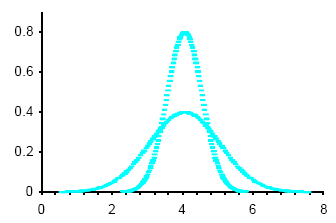
\includegraphics[width=0.3\linewidth]{fig/screenshot005}
	\label{fig:screenshot005}
\end{figure}
	\end{itemize}
\newpage	
	Con questa distribuzione gaussiana si può trovare l'integrale a partire dalla conoscenza delle $n$ misure, di $\mu$ e $\sigma_x$ calcolabili, ma è assai dispendioso calcolare ogni volta un integrale, non è meglio avere un andamento standardizzato, magari tabulato? Si ricorre ad un cambio di variabili per ottenere la distribuzione normale standardizzata.
	\[z_i = \dfrac{x_i-\mu}{\sigma_x}\]
	Per cui:
	\[\mu_z = \sum_{i}^{n}{z_i\over n} = {1\over n}\sum_{i}^{n}\dfrac{x_i-\mu}{\sigma_x} =  {1\over\sigma_xn}\left[\sum x_i - \sum\mu\right] \]
	Ricordando che sommare $n$ volte una costante significa moltiplicare per $n$ il valore della costante: 
	\[{1\over\sigma_xn}\left[\sum x_i - \sum\mu\right] = {1\over\sigma_xn}\left[\sum x_i - n\mu\right] = {1\over\sigma_x}\left[\mu - \mu\right] = 0\]
	Che si aggiunge al fatto che: 
	\[ \sigma_z = \sqrt{\dfrac{\sum(z_i - 0)^2}{n}} = \sqrt{{1\over n}\sum\left(\dfrac{x-\mu}{\sigma_x}\right)^2} = {1\over\sigma_x}\sqrt{\dfrac{\sum(x_i-\mu)^2}{n}} = {1\over\sigma_x}\sigma_x = 1 \]
	La curva distribuzione gaussiana standardizzata si può esprimere nella forma $N(0,1)$ ed è rappresentata dalla seguente funzione: 
	\[ y(z) = \dfrac{1}{\sqrt{2\pi}}e^{\dfrac{-z^2}{2}}\]
	$z$ altri non è che la distanza sull'asse delle ascisse misurato in unità di deviazioni standard. 
	
	Tale relazione evidenzia inoltre come la forma della distribuzione non dipenda più né dalla sua media né dalla sua varianza. \newline 
	
	Nella pratica statistica le proprietà più utili della distribuzione normale non sono i rapporti tra ascissa ed ordinata, bensì la relazione tra la distanza di un determinato valore $ x $ dalla media $\mu$ e la densità di probabilità (area) sottesa dalla curva. \newline 
	
	In questa distribuzione i punti si flesso si troveranno a $z = \pm 1$, quant'è l'area sottesa in questo intervallo? Si svolge banalmente l'integrale:
	\[\int_{-1}^{+1}y(z)dz = 68.3\%\]
	Ci si chiede a questo punto quanto valga la vecchia variabile nel punto di flesso: 
	\[z = \left.\dfrac{x-\mu}{\sigma_x}\right|_{z = 1} \Rightarrow x = \mu + \sigma_x\]
	\[z = \left.\dfrac{x-\mu}{\sigma_x}\right|_{z = -1} \Rightarrow x = \mu - \sigma_x\]
	Definendo:
	\[x = \mu \pm \sigma_x\]
	Ottengo che se faccio un'altra misura, al $ 68.3\% $ quella cadrà all'interno di quell'intervallo, mentre $\sigma_x$ indicherà la probabilità di avere una misura esterna, in questo caso pari al  $ 31.7\% $. 
\newpage	
	Sempre nella trattazione di intervalli simmetrici si ottiene che:
	\[\int_{-2}^{+2}y(z)dz = 95.5\% \Rightarrow \begin{aligned}
		\left.z\right|_{z = 2} & = \mu + 2\sigma_x \\
		\left.z\right|_{z = -2} & = \mu - 2\sigma_x 
	\end{aligned} \Rightarrow x = \mu \pm 2\sigma_x\]
	Ho il $ 95.5\% $ di sicurezza che la mia misura caschi all'interno dell'intervallo. \newline
	
	E ancora:
	\[\int_{-3}^{+3}y(z)dz = 99.7\% \Rightarrow \begin{aligned}
		\left.z\right|_{z = 3} & = \mu + 3\sigma_x \\
		\left.z\right|_{z = -3} & = \mu - 3\sigma_x 
	\end{aligned} x = \mu \pm 3\sigma_x \]
	Dare il $ \pm 3\sigma_x$ come incertezza significa dire che ho lo $0.3\%$ di probabilità che la misura caschi fuori dall'intervallo considerato. \newline 
		
	Si avrà infine: 
	\[x = \mu \pm z\sigma_x\]
	Dove $z\sigma_x$ altro non è che l'incertezza strumentale, legata allo strumento. \newline 
	
	Per minimizzarla si può scegliere di minimizzare la $\sigma_x$ e quindi di avere uno strumento maggiormente preciso e che garantista una maggiore ripetibilità, oppure si può aumentare $z$, questo deciso in modo da non incorrere in errori esageratamente elevati. 
\begin{figure}[H]
	\centering
	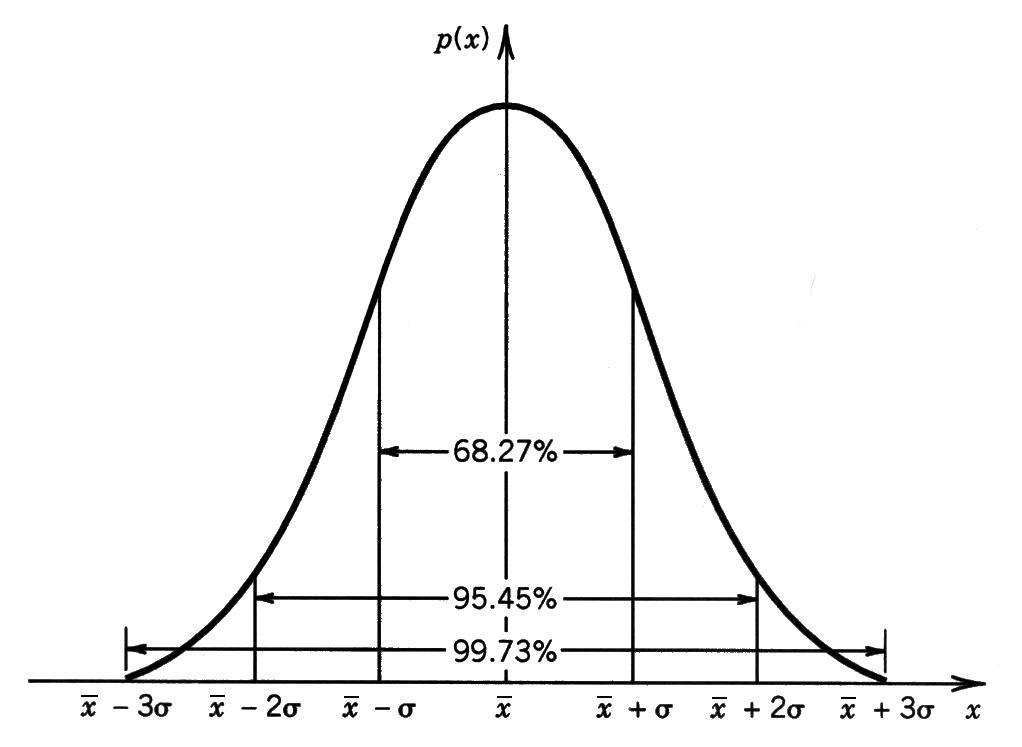
\includegraphics[width=0.5\linewidth]{fig/screenshot003}
	\label{fig:screenshot003}
\end{figure}	
\newpage
	La tabella di Gauss dà il valore dell'area esterna, le colonne sono la seconda cifra decimale di $z$ mentre le righe sono $z$ fino alla prima cifra decimale, i risultati che si ottengono entrando con $z$ nella tabella sono le aree esterne alla $z$ considerata, la significatività $\alpha$, per ottenere l'area interna, la confidenza $c$, basterà sottrarre all'unità la significatività. 
	\[c + \alpha = 1\]	
	\begin{figure}[H]
		\centering
		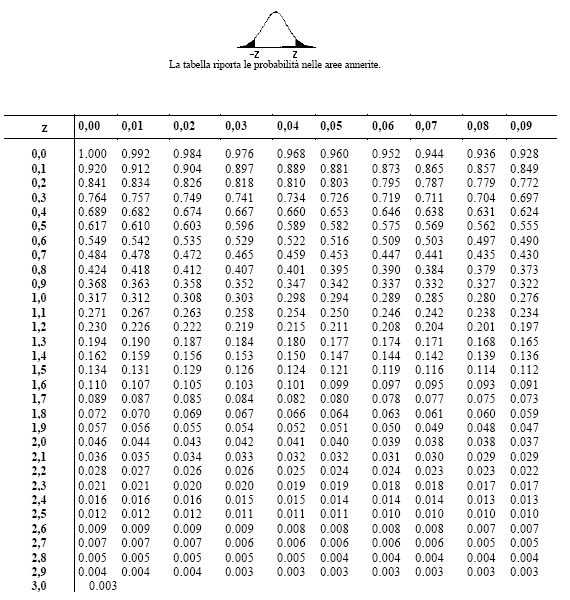
\includegraphics[width=0.7\linewidth]{fig/screenshot007}
		\label{fig:screenshot007}
	\end{figure}
	\textbf{Come si usa?} \\
	\textit{Esempio}:\\
	In una popolazione di studenti, l’altezza media $\mu$ è di 170 cm e la deviazione standard $\sigma_x$ è di 10 cm. Qual è la probabilità di trovare:	
	\begin{enumerate}		
	\item Studenti di altezza superiore a 180 cm?		
	\item Studenti di altezza compresa tra 180 cm e 190 cm?
	\end{enumerate}
	\begin{enumerate}
		\item \[\int_{180}^{\infty}y(x)dx \Rightarrow z(1) = \dfrac{x-\mu}{\sigma_x} = \dfrac{180-170}{10} = 1, z(\infty)=\infty \Rightarrow \int_{1}^{\infty}y(z)dz \]
\begin{figure}[H]
	\centering
	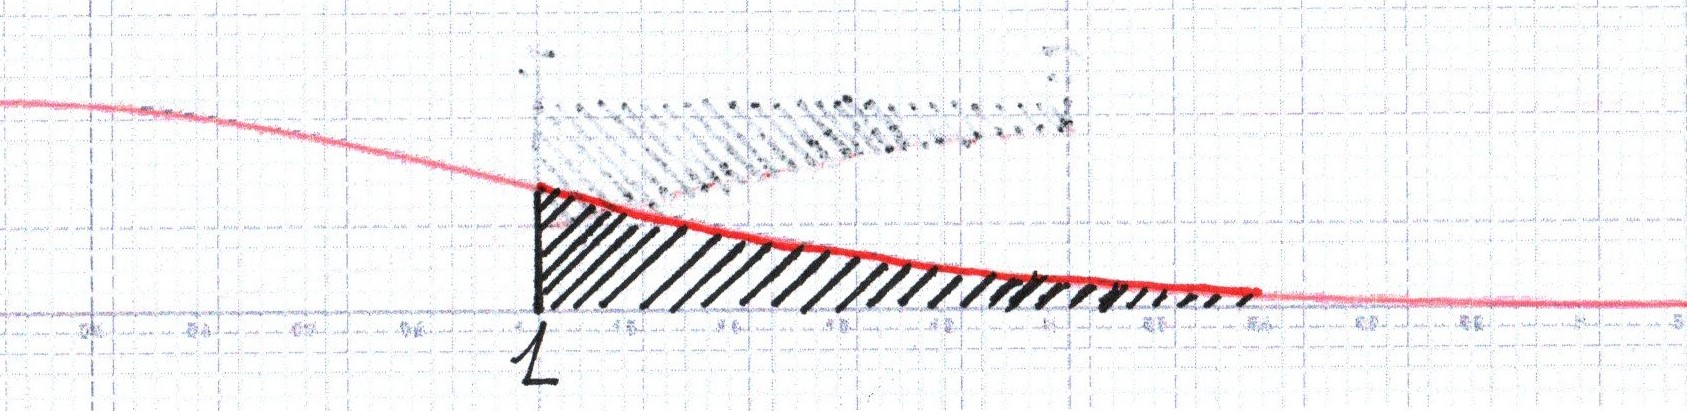
\includegraphics[width=0.5\linewidth]{fig/mm1}
	\label{fig:mm1}
\end{figure}
		In tabella vedo che $z=1$ l'area esclusa è $0.317$ essendo l'area di entrambe le ali dividendo per due si ottiene una probabilità del $15.85\%$. 
\newpage		
		\item \[\int_{180}^{190}y(x)dx \Rightarrow z(180) =  1, z(190)=2 \Rightarrow \int_{1}^{2}y(z)dz\]
\begin{figure}[H]
	\centering
	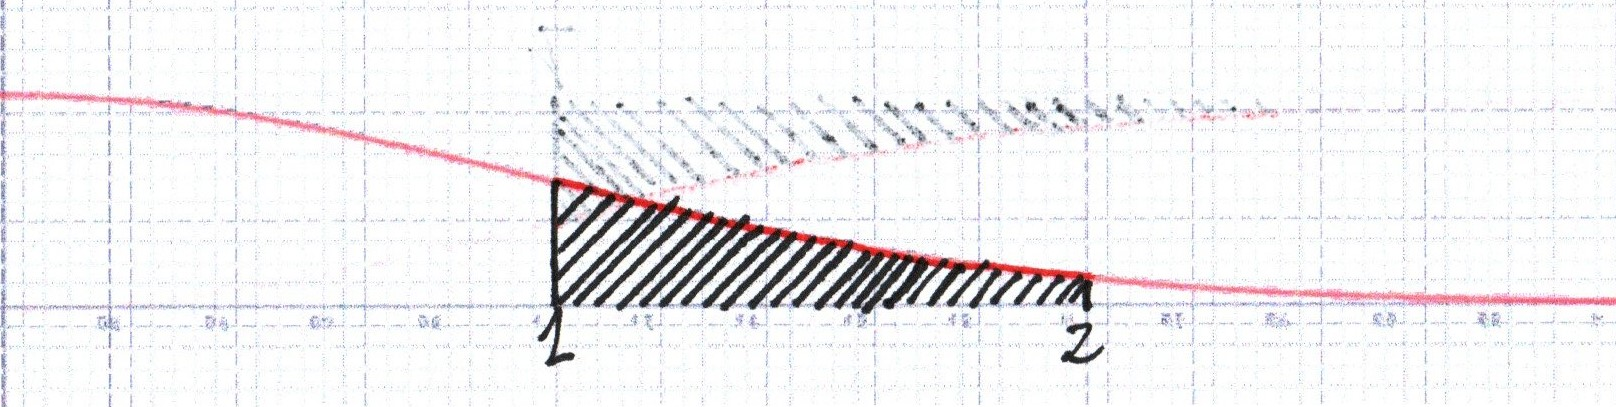
\includegraphics[width=0.5\linewidth]{fig/mm2}
	\label{fig:mm2}
\end{figure}		
		In tabella ottengo che per $z=1$ l'area esclusa è $0.317$ mentre per $z=2$ l'area esclusa è $0.046$, ottengo perciò \(\dfrac{0.317 - 0.046 }{2} = 13.5\%\)
	\end{enumerate}
\end{adjustwidth}
%\newpage
\section{Deviazione standard del valor medio}
\begin{adjustwidth}{2in}{}	
	Che succede se rimuovo un'ipotesi dal modello iniziale di Gauss? 
	
	Che succede se $\mu\ne\overline{x}$?\newline 
	
	Sto ipotizzando che il campione considerato non coincida più con la popolazione, ma ho lo stesso un gran numero di misure per cui $s_x\approx\sigma_x$.\newline 
	
	Un problema in statistica è quello di desumere quanto si discosta la media del campione dalla media della popolazione. Per far questo si ipotizza di estrarre da una popolazione di dati aventi media $\mu$ una serie di sottogruppi di cui si calcolano le medie e le deviazioni standard. \newline
	
	Si identificano cioè $p$ campioni composti da $n$ misure di cui si calcoleranno le $\overline{x}_p$ medie fino ad ottenere la completezza della popolazione $n\times p$, di queste medie se ne calcolerà la media per cui si identificheranno:
	\[\overline{\overline{x}} = \mu\]
	\[\sigma_{\overline{x}} = \sqrt{\sum_{i}^{p}\dfrac{(\overline{x}_i -\mu)^2}{p}}\]
	Sempre sotto le ipotesi in cui $s_x\approx\sigma_x$, vale l'importante fatto che:
	\[ \sigma_{\overline{x}} =  \dfrac{\sigma_x}{\sqrt{n}}\]
	Questo risulta essere un indice di quanto il valor medio, determinato con una sola serie di misure, differisca dal valore vero della grandezza in esame.\newline
	
	Ci si chiede allora, come si distribuisce la media delle medie intorno al valor medio? \newline
	
	Si vuole trattare il problema come appena fatto con Gauss, ovvero standardizzandolo:
	\[z_i = \dfrac{\overline{x}_i - \mu}{\sigma_{\overline{x}}}\]
	Se si ha una media in più con che probabilità cade nell'intervallo considerato? 
	\[\overline{x} = \mu \pm z\sigma_{\overline{x}} \Rightarrow\overline{x} = \mu \pm z\dfrac{\sigma_x}{\sqrt{n}}\]
	Ovvero posso esprimere:
	\[\mu - z\dfrac{\sigma_x}{\sqrt{n}} \leq \overline{x}\leq \mu + z\dfrac{\sigma_x}{\sqrt{n}} \]
	Sebbene $\sigma_x, n, \overline{x}$ siano oggetti noti, la media della popolazione non lo è, e allora converrà riscrivere la precedente relazione in funzione dell'incognita.\newline
	
	Si definisce \textbf{livello di confidenza} ($ c $) la percentuale di probabilità che la media $\mu$ di una popolazione giaccia in un intervallo (intervallo di confidenza) compreso tra:
	\[\overline{x} - z\dfrac{\sigma_x}{\sqrt{n}} \leq \mu \leq \overline{x} + z\dfrac{\sigma_x}{\sqrt{n}} \]
	Dicendomi così con quale probabilità la media della popolazione (incognita) cade all'interno di un intervallo che si può calcolare: si può in questo modo estrarre un concetto sulla popolazione considerando i campioni! 	
	\[\mu = \overline{x} \pm z\dfrac{\sigma_x}{\sqrt{n}}\]		
	Ora il valore $z\dfrac{\sigma_x}{\sqrt{n}}$ è l'incertezza legata alla misura: d'altro canto si sta lavorando sulla popolazione. 
		
	Questa si può diminuire aumentando $n$, il numero delle prove, tant'è che per $n\rightarrow\infty$ l'incertezza è nulla, si sta analizzando l'intera popolazione. \newline 
	
	Oltre alla confidenza $c$ si è parlato del parametro $\alpha$, questo rappresenta il livello di significatività ossia la percentuale di probabilità che la media $\mu$ giaccia all’esterno di un dato intervallo. 	
	\begin{figure}[H]
		\centering
		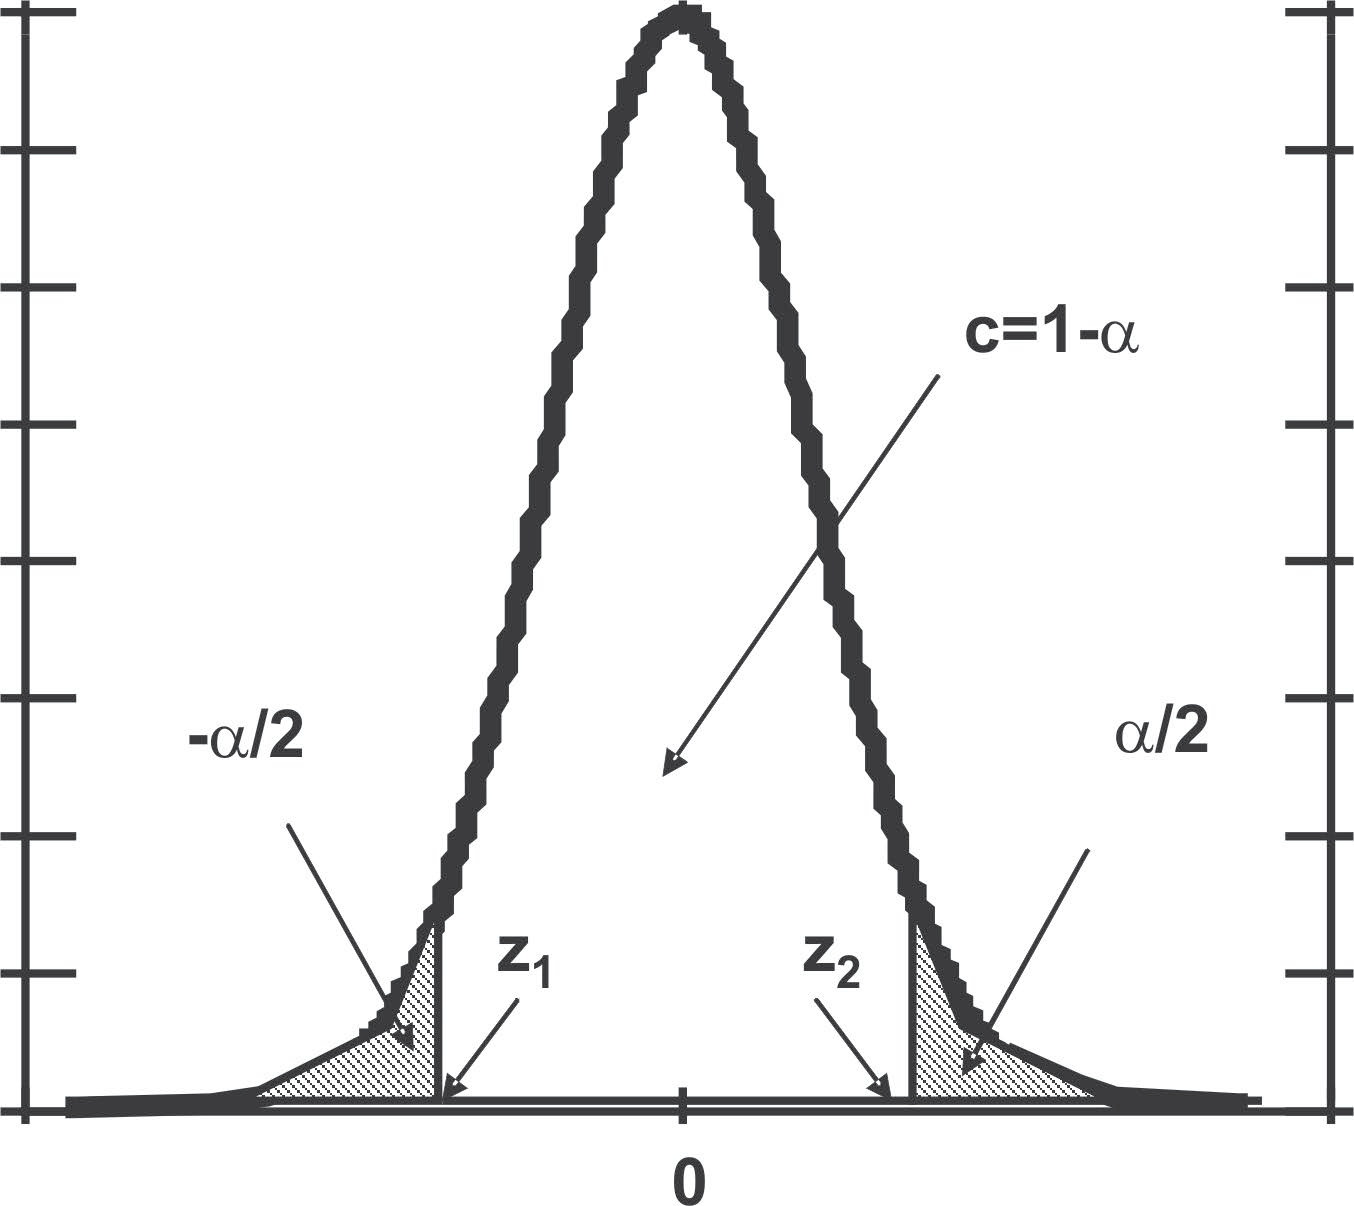
\includegraphics[width=0.5\linewidth]{fig/screenshot008}
		\label{fig:screenshot008}
	\end{figure}	
	Come si usa la tabella in questo caso? 
	
	Ad esempio si ipotizzi che per una data serie di $ n $ misure si sia calcolata la media $\overline{x}$ e la deviazione standard $ s_x $ ($s_x\approx\sigma_x$). Si vuole calcolare l’intervallo in cui cade la media dell’intera popolazione con una probabilità (livello di confidenza) del $ 95\% $. Per far questo si dovrà trovare dalla tabella il valore di $ z $ corrispondente a $ 0.05 $ ossia $ z=1.96 $. \newline 
\end{adjustwidth}
\newpage
\section{Distribuzione $t$ di Student}
\begin{adjustwidth}{2in}{}		
	E se oltre ad essere $\mu\ne\overline{x}$ si aggiungesse $\sigma_x\ne s_x$? Ovvero e se la deviazione standard del campione fosse diversa dalla deviazione standard della popolazione? \newline 
	
	Nella prassi della ricerca sperimentale, non sono note né la media della popolazione né la deviazione standard della popolazione. Tuttavia per un numero di misure superiore a 30 o 50 è possibile sostituire quest’ultima con la deviazione standard del campione. Nel caso in cui, invece, il numero di misure sia inferiore o uguale a 30 o 50, la distribuzione delle probabilità non è più fornita dalla distribuzione normale ma da quella del $ t $, detta $ t $ di Student, dallo pseudonimo di William Sealy Gosset. 
	
	All'aumento del numero di dati campionari, $ s $ è una stima sempre migliore di $\sigma_x$. Quando $ n $ è sufficientemente grande, $ s $ e $\sigma_x$ hanno valori praticamente identici. Di conseguenza all'aumentare di $ n $ si ha la convergenza dei valori della distribuzione $ t $ di Student verso la distribuzione normale standardizzata.\newline 
	
	In parole povere la distribuzione $t$ di Student è una correzione della curva di Gauss data dal fatto che $n$ diminuisce, questa è legata al grado di libertà ($gdl$ 0 $\nu$):
	\[gdl = \nu = n - ~ \text{vincoli}\]
	I vincoli sono equazioni che legano tra loro le misure. Poiché si sta prendendo in considerazione la media, il vincolo in questo caso è offerto dal fatto che la somma degli scarti è nulla, se si è definita \(\overline{x} = \sum\dfrac{x_i}{n}\) allora varrà che \(\sum\xi=0\), il numero di vincoli imposti è uno. \newline 
	
	Si ottengono una serie di curve parametrizzate a seconda del grado di libertà. 	
	\begin{figure}[H]
		\centering
		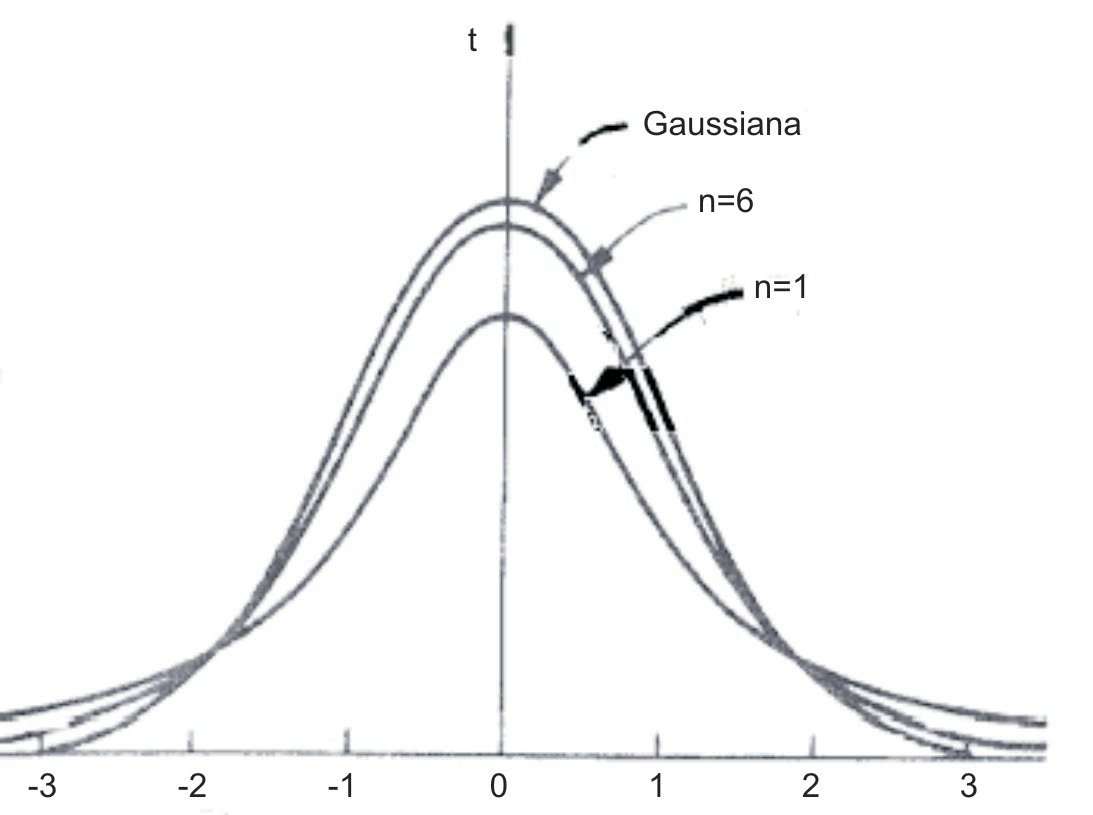
\includegraphics[width=0.5\linewidth]{fig/screenshot009}
		\label{fig:screenshot009}
	\end{figure}
	Si noti come tutte le curve corrette passino per i flessi della gaussiana e si abbassino gradualmente col diminuire delle misure e del $gdl$: l'area diminuisce, la media cade in quell'intervallo con una percentuale minore.\newline 
	
	Che fare per ottenere la stessa probabilità che avevo negli intervalli di Gauss? Dovrò avere un intervallo maggiore aumentando necessariamente l'incertezza: varia $z$, oltre che $n$!
	
	Utilizzare la gaussiana significa sottostimare l'incertezza del $t$ di Student.\newline 
	
	L'equazione della media della popolazione viene così riscritta con una nuova variabile $t$, funzione del grado di libertà:
	\[\mu = \overline{x} \pm t_{gdl}\dfrac{s_x}{\sqrt{n}}\]
	Anche in questo caso ci sarà una tabella per calcolare i valori di $t$ ma al contrario di $z$ questi valori saranno dipendenti dal numero di misure.  
\newpage	
	Nella tabella $\alpha$ indica l'area complementare all'intervallo considerato, la significatività, a cui si assocerà una percentuale; $\nu$ indica invece il grado di libertà, in questo caso $\nu = n-1$; all'interno della tabella si troverà il valore di $t$, il valore per cui si dovrà moltiplicare l'intervallo ottenuto da $z$. 	
	\begin{figure}[H]
		\centering
		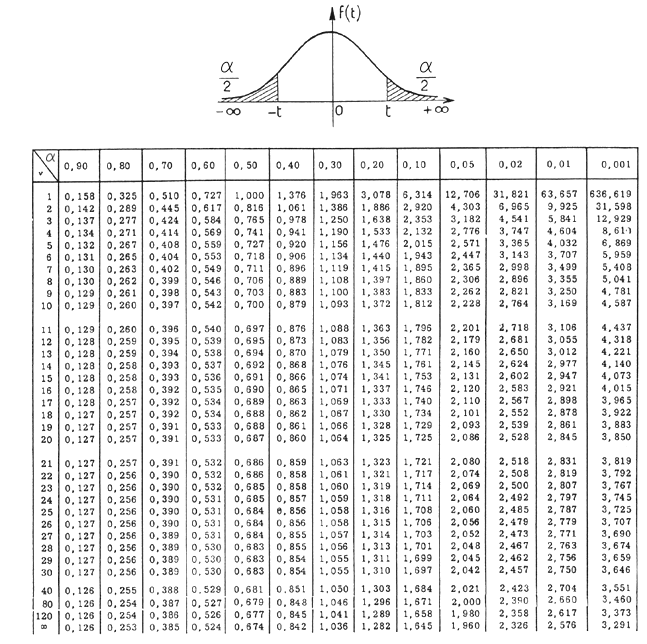
\includegraphics[width=0.7\linewidth]{fig/screenshot010}
		\label{fig:screenshot010}
	\end{figure}
\end{adjustwidth}
%\newpage
\subsection{Test di interferenza}
\begin{adjustwidth}{2in}{}	
	Alla base del $t$ di Student ci sono i test d'inferenza. Questi andranno sempre a decidere se due grandezze sono diverse tra loro, risponderanno alla domanda: Quanto è possibile considerare due grandezze differenti o uguali? Qual è la probabilità di sbagliare nel considerare due grandezze differenti o uguali? \newline 
	
	I test di interferenza sono principalmente 3: 
	\begin{enumerate}
		\item \textbf{Test sulle media}: confronto tra la media di un campione e la media attesa \newline
		Note $\mu$ $\overline{x}$ quante sono diverse tra loro? Se sono diverse tra loro è perché è successo un evento o non ho svolto la giusta quantità di misure? 
		
		\item \textbf{Test sul dato}: confronto tra un singolo dato e la media di un campione \newline
		Quanto una misura in più è diversa dalla media? 
		
		\item \textbf{Test su campioni differenti}: confronto tra le medie di due campioni differenti \newline 
		Se ho due gruppi di misure, quanto li possono considerare diversi tra loro? 
	\end{enumerate}
	Tutti i testi d'interferenza si basano su un'ipotesi nulla $H_0$, il test si compie vedendo che errore si commette nel rifiutare $H_0$. 
	
	Ci si chiede poi, quand'è che si può considerare accettabile l'errore? Lo decide lo sperimentatore, è la significatività $\alpha$ l'errore, questa rappresenta la probabilità che $\overline{x}$ sia lontano dalla media, voglio un $\alpha$ basso che mi dica se è accettabile o meno il risultato del test. 
	
	Ciò che si fa è dunque imporre un $\alpha_L$ limite, una significatività limite nel quale dovrà rientrare il test, si calcolerà poi attraverso dati noti $\alpha_m$, misurato e si vedrà se entra o meno nell'intervallo considerato. 	
\end{adjustwidth}
\newpage
\subsubsection{1. Test sulla media: test a due code}
\begin{adjustwidth}{2in}{}
		\[H_0: \mu = \overline{x}\]		
		Il test è a due code quando si vuole studiare se la media del campione è differente dalla media attesa. Il test è ad una coda nel caso in cui il confronto venga effettuato per vedere se la media del campione è unicamente minore oppure maggiore della media attesa.\newline 
		
		Che errore faccio nel rifiutare $H_0$? \(\mu \ne \overline{x}\)
		\[\mu = \overline{x} \pm t\dfrac{s_x}{\sqrt{n}}\]
		\[t = \dfrac{|\overline{x}-\mu|}{\dfrac{s_x}{\sqrt{n}}}\]
		Il primo passo che si compie è quello di imporre una significatività limite $\alpha_L$, così, noti i $gdl$, si troverà dalla tabella un $t_L$. 
		
		Il secondo passo è applicare l'equazione in $t$ appena ricavata per calcolare, attraverso dati noti, il $t_m$ misurato. \newline 
		
		Dopo aver svolto questi passaggi ci si troverà in due casistiche:
		\begin{enumerate}
			\item \[t_m>t_L \Rightarrow \begin{aligned}
				c_m&>C_L \\
				\alpha_m&<\alpha_L
			\end{aligned}\]
		
		Ero disposto ad accettare un errore addirittura maggiore! Supero il limite imposto positivamente. 
		
		Il risultato del test è positivo: posso considerare \(\mu \ne \overline{x}\) Cos'è successo tra il calcolo delle due medie? Sicuramente qualcosa. 
		
		\item \[t_m<t_L \Rightarrow \begin{aligned}
			c_m&<C_L \\
			\alpha_m&>\alpha_L
		\end{aligned}\]
	
		In questo caso l'esito del test è negativo non posso rifiutare l'ipotesi nulla, questo vuol dire che misure sono uguali tra loro? NO. 
		
		Non posso dire nè che sono uguali nè che sono differenti, se le considero uguali compio un errore del $c\%$. 
		\end{enumerate}	
		\textit{\underline{Esempio}}:\\
		In un vivaio sono coltivate piante della specie A; una lunga serie di misure ha dimostrato che tali piante, dopo due mesi dalla semina, raggiungono un’altezza media di 25 cm. A causa di una dispersione di sostanze tossiche si ritiene che esse incidano sulla crescita di alcune specie, tra le quali la specie A. Per una verifica di tale ipotesi vengono seminate sul terreno inquinato 7 pianticelle che, controllate dopo 2 mesi, raggiungono le seguenti altezze in cm.: 22, 25, 21, 23, 24, 25, 21.
		Si intende rispondere a due quesiti.
		Si può sostenere che le sostanze tossiche disperse influiscono sulla crescita della specie A con livello di confidenza pari al 90\%?
		Quale è la media reale dell’altezza delle piante dell’età di due mesi (media della popolazione), nella nuova condizione del terreno?  
		
		\textit{\underline{Risposta}}:\\
		Il test è a due code in quanto bisogna vedere se la media del campione è differente dalla media della popolazione. La significatività è $ \alpha=0,10 $ e la media dell’altezza delle piante $ x=23 cm  $ ed $ s=1,73 cm $. Il corrispondente in tabella è $ t_6=1,943 $. 
		
		Utilizzando ORA i dati dell’esercizio si ottiene un $ t $ stimato pari a:
		\[t_gdl=t_6 =  \dfrac{|23-25|}{1.73{\sqrt{7}}} = 3.053 \]
		Tale valore è superiore a quello riportato nella tabella sinottica della distribuzione $ t $, ci troviamo nel caso $(a)$.
		SI PUÒ dire, quindi con una confidenza maggiore del 95\% - e quindi con una significatività inferiore a 0.05 - che le sostanze tossiche disperse influiscono sulla crescita delle piante della specie A in modo significativo.
		
		L’altezza media reale della popolazione dalla quale sono stati estratti i sette dati può essere stimata considerando che ora il t da prendere in tabella è $ t_{0.10;6}=1.943 $:
		\[\mu = 23 \pm 1.943\dfrac{1.73}{\sqrt{7}} = 23.0\pm1.3\]
\end{adjustwidth}
%\newpage
\subsubsection{2. Test sul dato}
\begin{adjustwidth}{2in}{}		
\[H_0: x_{n+1} = \overline{x}\]	
	Ho un campione di misure a cui aggiungo una misura, questa $n+1$-esima misura fa ancora parte della distribuzione già calcolata? \newline 
	
	Che errore faccio nel rifiutare $H_0$? \(x_{n+1} \ne \overline{x}\)
	\[t = \dfrac{|\overline{x}-x_{n+1}|}{\dfrac{s_x}{\sqrt{\dfrac{N+1}{N}}}}\]
	Dove la quantità sotto radice altro non è che un fattore correttivo dato dal fatto che abbiamo una misura in più< la deviazione standard va ricalcolata. 
		\begin{enumerate}
		\item \[t_m>t_L \Rightarrow \begin{aligned}
			c_m&>C_L \\
			\alpha_m&<\alpha_L
		\end{aligned}\]
		
		L'esito del test è positivo.
		
		È successo qualcosa che ha reso la misura differente dalle altre: la misura in più non appartiene alla distribuzione delle altre misure. 
		
		\item \[t_m<t_L \Rightarrow \begin{aligned}
			c_m&<C_L \\
			\alpha_m&>\alpha_L
		\end{aligned}\]
		
		Il test è negativo, commetto un errore di $c\%$ nel considerare quella misura uguale alle altre. 
		\end{enumerate}
\end{adjustwidth}
%\newpage
\subsubsection{3. Test su campioni differenti}
\begin{adjustwidth}{2in}{}			
\[H_0: \overline{x}_1 = \overline{x}_2\]		
		Prendendo due campioni di misura, le medie sono diverse tra loro? Per quale motivo le medie vengono differenti? Per un evento particolare o perché non ho abbastanza misure? 
		
		In questo test il numero di misure per campione può essere differente, si suddivide in: 
		\begin{itemize}
			\item Dati non appaiati quando tra le misure dei due campioni non c'è alcuna relazione; 
			\item Dati appaiati, quando si ottengono misure diverse da campioni uguali in condizioni diverse e quindi c'è una relazione orizzontale tra le misure, si considera la variabilità di ogni soggetto. 
		\end{itemize}  
\newpage		
		\paragraph{Dati appaiati} \mbox{} \\ 
		\begin{table}[H]
			\centering	
			\begin{tabular}{|c|c|c|c|}
				\hline
				Soggetti & Condizione 1 & Condizione 2 &            Differenze             \\ \hline
				  $I$    &  $x_{I,1} $  &  $x_{I,2}$   &     $d_I = x_{I,1} - x_{I,2}$     \\ \hline
				  $II$   &  $x_{II,1}$  &  $x_{II,2}$  &  $d_{II} = x_{II,1} - x_{II,2}$   \\ \hline
				 $III$   & $x_{III,1}$  & $x_{III,2}$  & $d_{III} = x_{III,1} - x_{III,2}$ \\ \hline
				$\vdots$ &   $\vdots$   &   $\vdots$   &             $\vdots$              \\ \hline
				  $X$    &  $x_{X,1}$   &  $x_{X,2}$   &     $d_X = x_{X,1} - x_{X,2}$     \\ \hline
				 $\mu$   &              &              &          $\overline{d}$           \\ \hline
			\end{tabular}
		\end{table}
		
		Dove $d$ è null'altro che la differenza con segno. 
		
		Cambio soggetto dell'analisi statistica, ora non è più la media del campione ma la media delle differenze $\overline{d}$!
		
		La nuova ipotesi nulla che ottengo è: \[H_0: d = 0\]		
		Che errore faccio nel rifiutarla? 
		\[t = \dfrac{|\overline{d}-\delta|}{\dfrac{s_d}{\sqrt{n}}}\]
		Dove $\delta=0$ ed $n$ è ora il numero delle differenze. 
		
		Anche qui, se:
		\begin{enumerate}
			\item \[t_m>t_L \Rightarrow \begin{aligned}
				c_m&>C_L \\
				\alpha_m&<\alpha_L
			\end{aligned}\]
			
			L'esito del test è positivo. Rifiuto $H_0$ e la differenza $d\ne0$ è non nulla: le due medie sono diverse tra loro 
			
			\item \[t_m<t_L \Rightarrow \begin{aligned}
				c_m&<C_L \\
				\alpha_m&>\alpha_L
			\end{aligned}\]
			
			Il test è negativo, NON rifiuto l'ipotesi nulla ma questo non vuol dire che la differenza $d$ sia nulla! Significa semplicemente che non si può rifiutare l'ipotesi nulla con la data significatività limite imposta. 
		\end{enumerate}
	\textbf{(Dati non appaiati: NO)}	
\end{adjustwidth}
\newpage
\section{Retta di regressione}
\begin{adjustwidth}{2in}{}		
	Ricordi la differenza tra curva di graduazione e quella di taratura? Se la curva di graduazione era la caratteristica dello strumento, quella di taratura meglio approssima lo strumento e si ricostruisce dando ingressi noti allo strumento. \newline 
	
	Si definisce una relazione di regressione tra ingresso e uscita, una relazione del tipo semplice polinomiale:
	\[ y = a_0 + a_1x + a2x^2 + \dots +a_nx^n\]
	La \textbf{regressione lineare} è definita come una sola uscita $y$ dipendente da un solo ingresso $x$, un'equazione polinomiale di primo grado, una retta:
	\[ y = a + bx\]
	Occorre pertanto ricavare i due coefficienti $ a $ e $ b $, corrispondenti rispettivamente all’intercetta e all’inclinazione della retta. \newline
	
	Ora, ricordi perché si preferisce lavorare con curve lineari? Perché la sensibilità è costante: 
	\[S = {dy\over dx} = b\]
	In questo modo lo strumento si comporta nello stesso modo in tutto il campo di misura. \newline 
	
	Come si effettua una taratura? Dando ingressi noti se ne registra l'uscita. \newline
	
	Ad esempio per una bilancia $y=a+bx \rightarrow \theta = a+bF$. \newline
	
	Di quanti punti ho bisogno per tracciare una retta? Due, ma quando si hanno a disposizione $ n $ punti $ (X_i,Y_i) $ il sistema diviene sovradeterminato ($ 2xn $). 
	
	È necessario allora trovare una strategia di ottimizzazione per determinare la “migliore” retta
	che approssimi globalmente tutto l’insieme di punti a disposizione e che riduca le equazioni vincolari da $ n $ a $ 2 $. In generale tale strategia consiste nella minimizzazione di una funzione $g(y)$ detta
	\textit{errore ammissibile} o \textit{funzione obiettivo}.
	\[g(y) = \sum_{i=1}^{n}(y_i-\hat{y}_i)^2\]
	Questa è definita come la somma degli scarti verticali, dove $\hat{y}_i$ altro non sono che i punti appartenenti alla retta e gli $y_i$ sono quelli ottenuti dalla costruzione. \newline 
	
	Come trovo la retta che minimizzi tale funzione? Annullando le derivate parziali rispetto ad $a$ e $b$ (le uniche due quantità che variano).
	
	Sostituendo i punti sulla retta nell'equazione di $g$ ottengo: 
	\[g(y) = \sum_{i=1}^{n}(y_i-a-bx_i)^2\]
	Derivando si trova in questo modo gli unici due valori di $a$ e $b$ che minimizzano la funzione $g$: 
	\[ \begin{aligned}
		{\partial g\over \partial a} & = 0 \Leftrightarrow -2\sum(y_i - a - bx_i) = 0 \Leftrightarrow \\
		\sum y_i - \sum a - \sum bx_i & = \sum y_i - na - b\sum x_i = 0 \Leftrightarrow \sum {y_i\over n} - a - b\sum {x_i\over n} = 0 \Leftrightarrow \\
		\overline{y} - a - b\overline{x} & = 0 \Leftrightarrow \boxed{a = \overline{y} - b\overline{x}}
	\end{aligned}\]
	Si sostituisca quanto appena trovato nella formula di partenza di $g$:
	\[g(y) = \sum_{i=1}^{n} (y_i-\overline{y} - b\overline{x}-bx_i)^2 = \sum_{i=1}^{n}\left[y_i - \overline{y} - b(x_i - \overline{x})\right]^2\]
	Derivando:
	\begin{eqnarray*}
		{\partial g\over \partial b}  = 0 \Leftrightarrow -2\sum\left[y_i - \overline{y} - b(x_i - \overline{x})\right](x_i - \overline{x}) \Leftrightarrow \\
		\sum(y_i - \overline{y})(x_i - \overline{x}) - b\sum(x_i-\overline{x})^2  = 0 \Leftrightarrow \\
		\boxed{b = \dfrac{	\sum(y_i - \overline{y})(x_i - \overline{x})}{\sum(x_i-\overline{x})^2}} = {cod_{xd}\over dev_x}
	\end{eqnarray*}
	Dove $cod$ e $dev$ sono rispettivamente la codevianza e la devianza. \newline 
	
	\begin{center}
		\textbf{La retta di regressione lineare vale soltanto nel range di valori dati, non si può estendere la legge lineare trovata all'esterno dell'intervallo di valori considerato.}
	\end{center}
\end{adjustwidth}
%\newpage
\subsection{Test di significatività}
\begin{adjustwidth}{2in}{}	
	In quali casi non si può calcolare la retta di regressione lineare? Sempre, a patto di avere almeno due punti, è una relazione matematica. \newline 
	
	Il problema è capire quanto ciò che si calcola è indice o meno di linearità.
	\begin{figure}[H]
		\centering
		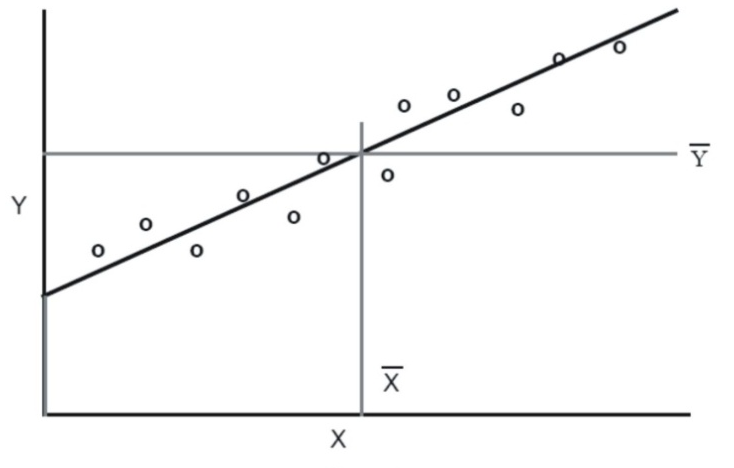
\includegraphics[width=0.5\linewidth]{fig/screenshot011}
		\label{fig:screenshot011}
	\end{figure}	
	Più $b$ si discosta da 0, più si può dire che sussiste una relazione di linearità tra ingresso ed uscita, ma non dipenderà soltanto dall'inclinazione $b$, ma anche dalla dispersione dei dati. 
\begin{figure}[H]
	\centering
	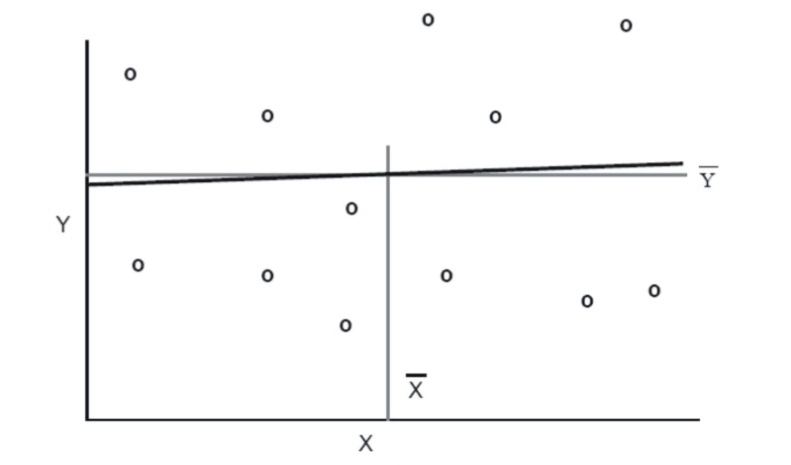
\includegraphics[width=0.5\linewidth]{fig/screenshot012}
	\label{fig:screenshot012}
\end{figure}
	Questo è ad esempio uno strumento poco sensibile ma pur sempre lineare.
	
	Ci si chiede allora se il risultato dell'avere un $b$ piccolo è causato dall'avere uno strumento dalla bassa sensibilità o perché se si avessero fatte più misure allora $b\rightarrow0$? \newline 
\end{adjustwidth}
%\newpage
\subsubsection{Test di linearità}
\begin{adjustwidth}{2in}{}		
	Occorre determinare quindi quale è la soglia inferiore accettabile di $ b $ per asserire la linearità
	del campione. L'analisi che si effettuerà sarà soltanto sul coefficiente $b$. Tale test dirà pertanto se sussiste una relazione lineare, ma non darà informazioni sulla migliore approssimazione dei dati, che può essere quadratica, cubica, etc \dots. \newline 
	
	Dall'equazione della retta $\hat{y} = a + bx$ ci si chiede quanto $b$ sia non nullo, l'ipotesi nulla sarà pertanto \[H_0: b=0\]	
	Che errore si commette nel rifiutarla? Si rifiuti $H_0$ con un limite di significatività $\alpha_L$. Si esegua il test $t$ di Studenti su $b$: 
	\[t_m = t_{gdl} = {b-0\over S_b}\]
	Dove $S_b$ è la deviazione standard di $b$ così calcolata:
	\[S_b = \sqrt{\dfrac{\sum(y_i - \hat{y}_i)}{\sum(x_i-\overline{x}^2)}}\]
	In cui il termine al numeratore altro non è che la deviazione standard degli errori, in qui gli $ \hat{y}_i $ si calcolano dalla formula della retta. \newline 
	
	Quanti sono i gradi di libertà $gdl$? Valendo sempre:
	\[gdl = ~ \text{numero di misure} ~ - ~ \text{vincoli}\]
	In questo caso i vincoli sono due e sono offerti dalle condizioni di nullo delle derivate parziali in $a$ e $b$: 
	\[gdl = n - 2\]
	Ad esempio se si vuole essere sicuri al 95\% ($c_L = 95\% \Rightarrow\alpha_L = 5\%$) si calcola il corrispettivo $t_L$ e lo si confronterà con il $t_m$.
	
	\begin{enumerate}
		\item \[t_m>t_L \Rightarrow \begin{aligned}
			c_m&>C_L \\
			\alpha_m&<\alpha_L
		\end{aligned}\]
		
		L'esito del test è positivo, il test è significativo, superato. Si può rifiutare $H_0$ e si può considerare $b\ne0$: si può considerare la dipendenza lineare piuttosto che non avere dipendenza. 
		
		\item \[t_m<t_L \Rightarrow \begin{aligned}
			c_m&<C_L \\
			\alpha_m&>\alpha_L
		\end{aligned}\]
		
		Il test è negativo, non significativo non si può rifiutare l'ipotesi nulla con quella confidenza dichiarata. Tuttavia non si può neanche dire che $b$ sia nulla! 
		
		Vorrà dire che la relazione lineare cè ma non è così forte da stabilirsi con quella $\alpha_L$ data.
	\end{enumerate}
	\textbf{(Significatività dell’intercetta $ a $: NO) } 
\end{adjustwidth}
\newpage
\subsubsection{Test di parallelismo}
\begin{adjustwidth}{2in}{}		
	La retta di regressione $y = a +bx$ è parallela ad un'altra retta se presenta lo stesso coefficiente angolare/pendenza $b$, ma cosa significa per due rette di regressione avere in questo caso la sessa pendenza? Avere la stessa sensibilità.\newline  
	
	Magari se lo strumento ha subito danni il nuovo $b$ potrà essere differente dal vecchio, di quanto la sensibilità dello strumento è compromessa? Sono diversi perché un evento li ha resi tali o perché non sono state effettuate il numero sufficiente di misure? 	
	\[ y = a + bx \hspace{1cm} y = a + \beta x\]
	Quanto $b=\beta$?\newline 
	
	Con il test di parallelismo si deve rispondere alla seguente domanda:\textit{ è possibile affermare, con un livello di significatività $\alpha$, che i due coefficienti angolari
	$ b $ e $\beta$ sono diversi?}
	\begin{enumerate}[label=(\alph*)]
		\item Se il test risulta essere positivo, i due coefficienti sono significativamente
		diversi con un livello di significatività $\alpha$.
		\item Se il test è negativo, NON si può affermare che i due coefficienti sono uguali
		ma unicamente che i due coefficienti non sono significativamente differenti tra
		loro con il livello di significatività $\alpha$ scelto.
	\end{enumerate}
	Se si ricade nel caso (a) l’elemento oggetto della taratura (trasduttore/catena di misura) ha una sensibilità diversa da quella di riferimento. 
	
	Se si ricade invece nel caso (b) si può confidare che le due sensibilità siano uguali tuttavia, non essendo possibile affermarlo con certezza, è
	necessario formulare una seconda domanda \textit{è possibile considerare i due coefficienti “poco differenti” per gli scopi della misura?} \newline
	
	Per rispondere alla prima domanda, come per il test di linearità, si utilizza il test di Student.
	
	Con il valore di $ t $ infatti è possibile valutare la probabilità $\alpha_{(tn-2)}$ che$  b $ sia
	significativamente diverso da un dato valore atteso $\beta$. Tale probabilità corrisponde all'area
	sottesa dalla distribuzione $ t $ di Student esterna a $ -t $ e $ t $.\newline
	
	Tutti i test di inferenza analizzati finora, dalla loro definizione, si adoperavano a negare una condizione e pertanto venivano usati per quantificare quanto due grandezze fossero differenti. In questo caso, l'approccio è il contrario. \newline
	
	L'ipotesi nulla è data da: \[ H_0: b = \beta\] Con $\beta$ valore noto. 
	
	Quel che si fa questa volta, ragionando al contrario, è scegliere un $\alpha_L\Uparrow$ in modo da avere un $c_L\Downarrow$: si vuole "sbagliare", si vuole \textit{NON-rifiutare} l'ipotesi nulla, si vuole essere sicuri che le due grandezze siano uguali al $\alpha\%$ più alto possibile e differenti al $c\%$ più basso possibile. \newline

	Per cui: 
	\[t_m = t_{gdl} = \dfrac{\left|b-\beta\right|}{S_b}\]
	Mentre il $t_l$ si troverà imponendo questa volta un elevato valore di $\alpha_L$.
	
	\begin{enumerate}
		\item \[t_m>t_L \Rightarrow \begin{aligned}
			c_m&>C_L \\
			\alpha_m&<\alpha_L
		\end{aligned}\]
		
		L'esito del test è positivo, il test è significativo. Si può rifiutare $H_0$ e si può considerare $b=\beta$: le due pendenze sono diverse al $c\%$. 
		
		\item \[t_m<t_L \Rightarrow \begin{aligned}
			c_m&<C_L \\
			\alpha_m&>\alpha_L
		\end{aligned}\]
		
		Il test è negativo, non significativo non si può rifiutare l'ipotesi nulla con quella confidenza dichiarata. Si può sbagliare di un $\alpha\%$ a non considerarle uguali. 
		
		Si può considerare $b=\beta$ con quel livello di significatività dichiarato. 
	\end{enumerate}
	\textbf{SOLO se il test è NON significativo}, si potrà rispondere alla seconda domanda e considerare le uscite dei due trasduttori. 
	
	Si effettuerà cioè un controllo misuristico chiedendosi se l'errore fatto nello step di test precedente si può accettare a livello di utilizzo: il test non è uno strumento in grado di accertare
	l’uguaglianza tra le sensibilità, per cui si procede a considerare il massimo errore che si
	ottiene a causa della differenza esistente tra la sensibilità ottenuta e quella nominale.
	
	Si continui ad ipotizzare $a$ in prima approssimazione uguale, in modo che: 
	\[ y = a + bx \hspace{1cm} y'= a + \beta x\]	
\begin{figure}[H]
	\centering
	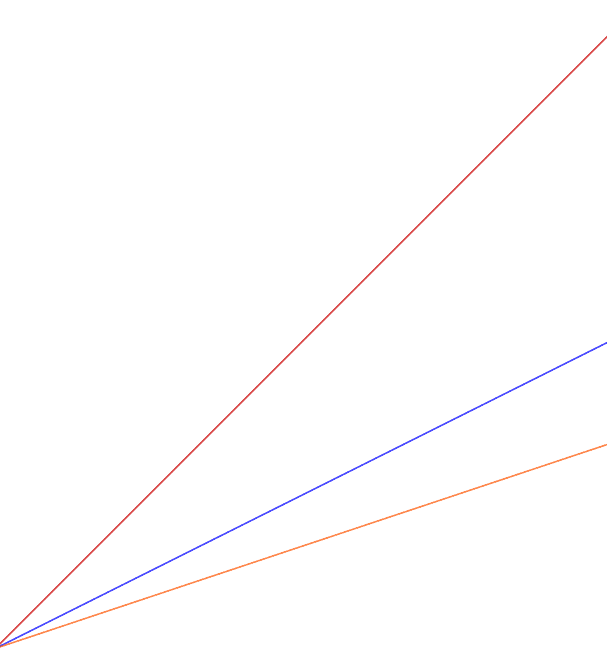
\includegraphics[width=0.3\linewidth]{fig/rettine}
	\label{fig:rettine}
\end{figure}	
	In ogni caso, che sia $\beta\gtrless b$ l'errore massimo sarà sempre in corrispondenza del massimo valore di ingresso $x_{max}$, l'errore $\Delta y$ che ne consegue può essere ricavato, a livello teorico: 
	\[\Delta y = \left|y-y'\right| = \left|b-\beta\right|x\]
	In questo modo a livello misuristico l'errore massimo si potrà scrivere come:
	\[\Delta y_{\max, \text{misurato}} = \left|b-\beta\right|x_{\max}\] 
	Tale risultato dovrà essere confrontato con un valore noto (dato dall'esercizio) per vedere se è accettabile o meno. 
	
	Poiché interessa sapere il valore sul misurando, sull'ingresso, verrà fornito un $\Delta x_{\max} $, nominale che dovrà essere confrontato con un $\Delta x_{\max, \text{misurato}}$:
	\[\Delta x_{\max, \text{misurato}} = \dfrac{\Delta y_{\max}}{\beta}\]
	
	Oppure, equivalentemente, si possono calcolare i valori massimi delle rette di regressione, ua nominale e l'altra modificata, ottenendone un $\Delta$, tale valore può essere poi ricondotto nelle unità di misura del misurando attraverso il valore o l'espressione della sensibilità nominale. 
		
	\textbf{(Intervallo di confidenza: NO)
	}
	
\newpage

{\LARGE \textbf{NOTE}}
	
	%DA DECOMMENTARE PER AVERE LA VERSIONE STAMPABILE A DUE PAGINE 	
	%	\newpage
	%		\null
	%		\vfill
	%\begin{tcolorbox}[height=4.5cm]
	%	This box has a height of 4.5cm.
	%\end{tcolorbox}
	%		
\end{adjustwidth}
\end{document}